\section{Análise Teórica}

Como os circuitos das figuras \ref{ckt:1} e \ref{ckt:2} constituem filtros de Butterworth de primeira e segunda ordem, devemos notar que ambos os circuitos são ativos devido a presença do buffers na suas respectivas saídas. Para analisar tais circuitos devemos primeiro obter as suas frequências de corte ($f_o$), pela suas funções de transferência T(s).

Para o filtro de primeira ordem de Butterworth, podemos calcular analisando T(s), onde podemos obter.


\begin{equation} \label{Ts}
T(s) = \frac{1}{1+RCs} = \frac{1}{1+150\times10^6s} 
\end{equation}

Podemos observar pela equação \ref{Ts} $k=1$ e  $w_o= \frac{1}{RC}$, logo poderemos obter $f_o$.

\begin{equation} \label{f1}
w_o = \frac{1}{RC} = \frac{1}{15\times 10^3 . 10 \times 10^{-9}}  = 6666,7 \hspace{6pt} rad/s
\end{equation}

\begin{equation} \label{f3}
f_o = \frac{w_o}{2\pi} = \frac{1}{2\pi  .RC} = \frac{1}{2\pi . 15\times 10^3 . 10 \times 10^{-9}} = 1,061 \hspace{6pt} kHz
\end{equation}


É possível notar que o ganho k em dB será nulo, logo o circuito não amplifica para frequências abaixo de $f_o$. Podemos traçar as curvas de bode de amplitude e fase para notamos o efeito mais importante do filtro que é o de atenuar a saída em -20dB/dec para frequências acima de $f_0$.

\begin{figure}[H] 
\centering
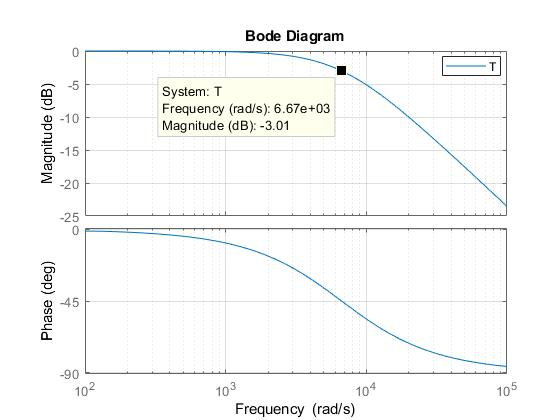
\includegraphics[width=12cm]{images/bode1ordem.jpg}
\caption{Diagrama de bode para o filtro de Butterworth de 1ª ordem obtido no MATLAB.}
\label{fig:20} 
\end{figure}

A partir dos gráficos da figura \ref{fig:20}, podemos notar na frequência de corte ($f_o$) o circuito tem aproximadamente -3dB de ganho na amplitude e uma fase de -45º. Portanto nesse ponto o circuito apresentará uma $V_o = 0.707V_{in}$.

Agora analisando o circuito da figura \ref{ckt:2}, ou seja um filtro de Butterworth de 2ª ordem, podemos representar o circuito pela a função de transferência abaixo.

\begin{equation} \label{Ts2}
    T(s) = \frac{w_o^2}{s^2+ \frac{w_o}{Q}s + w_o^2} = \frac{36.954\times10^6}{s^2+ 8574.11s + 36.954\times10^6}
\end{equation}

Onde $w_o$, $f_o$ e Q são:

\begin{center}
    $w_o = \frac{1}{\sqrt{R_1 R_2 C_1 C_2}} = \frac{1}{\sqrt{8,2 \times 10^3 15 \times 10^3 22 \times 10^{-9} 10 \times 10^{-9}}} = 6079, 06 \hspace{6pt} rad/s$
\end{center}




\begin{equation} \label{r}
    f_o = \frac{w_o}{2\pi} =  \frac{6079,06}{2\pi} = 967,51 \hspace{6pt} Hz
\end{equation}

\begin{center}
    $Q = C_1 \times (R_1 || R_2) \times w_o \approx 0,709$
\end{center}

Com os parâmetros obtidos podemos traçar a curva de bode para o filtro de 2ª ordem pela sua função de transferência. Portanto,

\begin{figure}[H] 
\centering
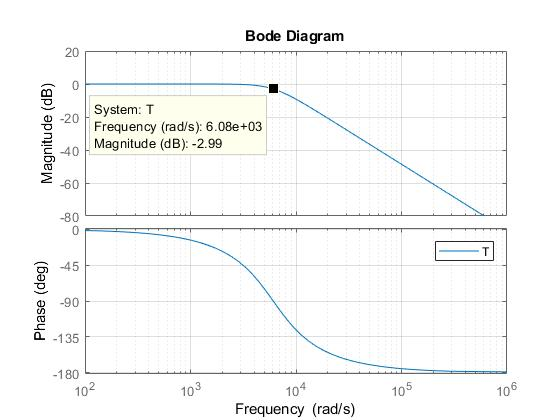
\includegraphics[width=12cm]{images/bode2ordem.jpg}
\caption{Diagrama de bode para o filtro de Butterworth de 2ª ordem obtido no MATLAB.}
\label{fig:4} 
\end{figure}


É possível notar que o ganho k em dB não será zero, logo o circuito amplifica/atenua para frequências em torno de $f_o$. pelas as curvas de bode de amplitude nota-se a tensão de entrada é atenuada em -40dB/dec para frequências acima de $f_0$.

Percebe-se ainda que em $f_o$ os valores serão de -3dB para magnitude, ou seja $V_o=0,707V_{in}$. E para a fase é de -90º. Nota-se também que os filtros de 2ª ordem são muitos suscetíveis ao fator Q, tendo grandes mudanças com alteração deste valor, veremos melhor esse efeito na seção seguinte.

